\subsubsection*{7) Virtualization}
\textbf{Virtualization:} abstraction of \textbf{hardware} (CPU, mem, I/O) for multiple isolated \textbf{environments (VMs)}. Overcomes \textbf{multicomputer model} limits (standalone machines) by combining reliability, isolation (sandboxing), and flexibility. \textbf{Benefits:} Dev/prototype ease, snapshots, migration, multi-OS on single machine.

\textbf{Components:} \textbf{Host} (HW), \textbf{Hypervisor (VMM)} (creates/manages VMs), \textbf{Guest} (process with virtual HW view).

\textbf{Types:} \textbf{Type 0} (\textbf{firmware partitions/domains}), small feature set (e.g., IBM LPAR). \textbf{Type 1} (native, datacenters, e.g., \texttt{ESXi}), runs in kernel mode, manages OSes, snapshots, cloning, balancing load. \textbf{Type 2} (hosted, e.g., \texttt{VirtualBox}), runs as a process on host OS, higher latency. Compare: \textbf{Type 1} → low latency, needs HW support, service providers; \textbf{Type 2} → high latency, no HW req., end-users. \textbf{Emulation:} diff. ISA, slow (e.g., Rosetta). \textbf{Paravirtualization:} modify guest OS to avoid traps.

\textbf{Building Blocks:} \textbf{VCPU} stores guest state, switched by VMM. \textbf{HW support} essential (e.g., \texttt{Intel VT-x}, \texttt{AMD-V}), incl. nested page tables, DMA, interrupts. \textbf{Trap \& Emulate:} guest runs in \textbf{virtual user/kernel mode} (both in HW user mode); traps on priv. instr. \textbf{Binary Translation:} rewrites priv. instr. on CPUs w/o clean separation. \textbf{Emulation:} simulates different ISA, slow. \textbf{HW Resources:} CPU, GPU, NIC, PCI, I/O devices.

\textbf{Paravirtualization:} modify guest OS to avoid traps.

\textbf{Programming Env VM:} e.g., \texttt{JVM} abstracts exec. env., cross-OS portability.

\textbf{Containers:} App-level isolation via \textbf{OS namespaces}; each has own FS, net stack, users. Lightweight, fast start, no full OS. \textbf{Docker}: \textbf{Image} (layers: e.g., Ubuntu, Python), \textbf{Container} (instance), \textbf{Engine}, \textbf{Registry}. Shared layers reduce redundancy. \textbf{Container Features:} app isolation, shared kernel, fast startup, low resource. \textbf{Limitations:} less isolation, security depends on user. Compare VMs vs Containers: \textbf{VMs} heavy, slow, full OS, hardware virt.; \textbf{Containers} light, fast, process-level isolation, share OS.

\textbf{CPU Scheduling:} VMM schedules VCPUs on physical CPUs; \textbf{overcommit} = more VCPUs than CPUs.

\textbf{Memory Mgmt:} VMM mediates guest/host mem; uses nested page tables. \textbf{Overcommit:} total guest alloc $>$ physical mem. VMM uses own paging, replacement.

\textbf{Storage:} VMs see \textbf{disk images} (Type 1 = VMM FS, Type 2 = host FS). \textbf{P2V/V2P} convert disk formats. VMM handles net disks.

\textbf{Live Migration:} Copy running VM incl. CPU state, memory pages (iterative dirty page copy); no disk state (remote disks for portability). \textbf{MAC mobility} requires network switch support.

\textbf{Container Problems Solved:} \textbf{VM CapEx/OpEx} (licenses, OS overhead) → Containers = low-cost, fast deploy. \textbf{Application Containment:} consistent, portable env; auto-packages apps + dependencies.

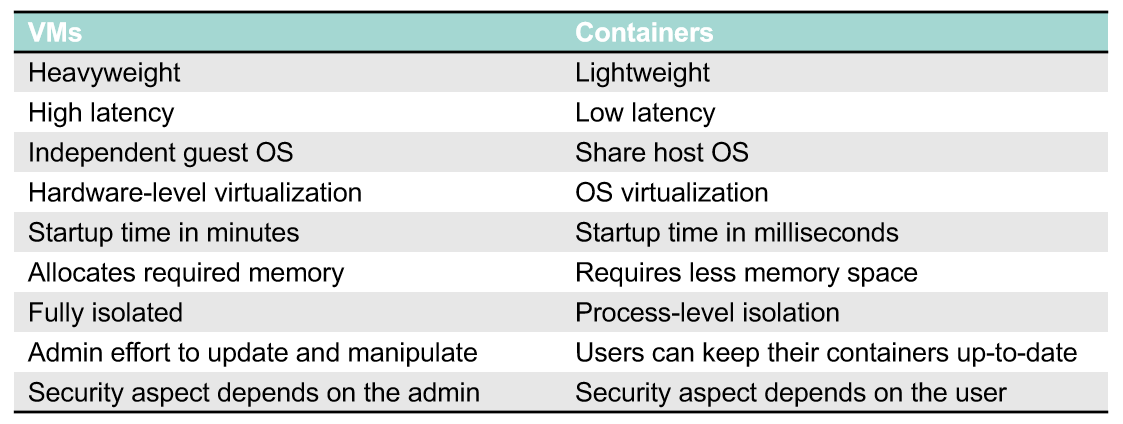
\includegraphics[width=0.95\linewidth]{images/07_p41_vm_vs_cont.png}

% \textbf{Virtualization vs Containerization}
% 1 HW-level abstraction vs. OS-level abstraction
% 2 Each VM has full OS vs. Containers share host kernel
% 3 Slow startup (minutes) vs. Fast startup (milliseconds)
% 4 Heavyweight (more resources) vs. Lightweight (less resources)
% 5 Full OS isolation vs. Process-level isolation
% 6 Hypervisor (VMM) manages VMs vs. Container Engine manages containers
% 7 Higher CapEx/OpEx (licenses, OS) vs. Lower CapEx/OpEx
% 8 Stronger isolation (security) vs. Weaker isolation (shared kernel)
% 9 Suitable for infra (e.g., IaaS) vs. Suitable for apps (e.g., microservices)